\documentclass[10pt,a4paper]{article}

\usepackage[margin=22mm]{geometry}
\usepackage[T1]{fontenc}
\usepackage[utf8]{inputenc}
\usepackage{lmodern}
\usepackage{microtype}
\usepackage{amsmath,amssymb,amsthm,mathtools}
\usepackage{booktabs,tabularx,array}
\usepackage{graphicx}
\graphicspath{{output/pdf/}{../../output/pdf/}}
\usepackage{tikz}
\usetikzlibrary{arrows.meta,positioning}
\usepackage{xcolor}
\usepackage[hidelinks]{hyperref}

\hypersetup{
  pdftitle={An Exact Chordal-Ordering QUBO for the Steiner Tree Problem},
  pdfauthor={Daghan Erdonmez}
}

\definecolor{navy}{HTML}{173B57}
\definecolor{blue}{HTML}{2E78A6}
\definecolor{orange}{HTML}{D66A4C}

\setlength{\parindent}{0pt}
\setlength{\parskip}{4pt}
\renewcommand{\arraystretch}{1.14}
\raggedbottom

\newtheorem{theorem}{Theorem}
\newtheorem{lemma}{Lemma}
\newcommand{\A}{\mathcal A}
\newcommand{\C}{\mathcal C}

\title{\textbf{An Exact Chordal-Ordering QUBO\\for the Steiner Tree Problem}}
\author{Da\u{g}han Erd\"onmez\\
\small Department of Computer Engineering, Bo\u{g}azi\c{c}i University}
\date{October 2026}

\begin{document}
\maketitle

\begin{abstract}
An existing ordering-based QUBO formulation for the Steiner Tree Problem
prevents cycles by ordering every pair of nonroot vertices. Although exact,
this construction requires $O(n^2)$ ordering variables and $O(n^3)$ ordering
interactions. We present an exact sparsification based on chordal completion.
The new formulation introduces ordering variables only on the edges of a
chordal completion of the nonroot graph and checks only the triangles of that
completion. For an elimination order of width $w$, the ordering part uses
$O(nw)$ variables and $O(nw^2)$ triangle interactions, while retaining the
same worst-case complexity as the complete-order formulation. We also give a
degree-local replacement for the original global nonterminal coefficient.
Exhaustive checks confirm the zero-penalty set on small graphs. Experiments on
350 generated instances and 18 SteinLib B instances show that the chordal
model is substantially smaller and more likely to produce valid trees when
the completion is sparse. Improvements in best-tree cost are less consistent
and depend on the graph family and solver.
\end{abstract}

\section{Introduction}

Let $G=(V,E)$ be an undirected graph with nonnegative edge costs, and let
$T\subseteq V$ be a set of terminal vertices. The Steiner Tree Problem asks
for a minimum-cost tree that connects all vertices in $T$. The tree may also
contain vertices in $V\setminus T$, called \emph{Steiner vertices}, when their
inclusion reduces the total cost~\cite{hwang1992}. The decision version is
NP-complete, and the corresponding optimization problem is therefore
NP-hard~\cite{karp1972}. Applications include communication, transportation,
and other network-design problems~\cite{hwang1992}.

Quadratic Unconstrained Binary Optimization (QUBO) expresses a combinatorial
optimization problem as a quadratic function of binary variables. Constraints
are represented by penalties that increase the energy of invalid assignments.
The resulting model can be processed by general-purpose QUBO solvers,
including simulated annealing and quantum annealing~\cite{glover2019,lucas2014}.
For such solvers, a formulation is influenced not only by whether its global
minimum is correct, but also by its number of variables, interaction density,
coefficient range, and distribution of infeasible states.

Fowler proposed an ordering-based QUBO for the Steiner Tree Problem that
directs selected edges away from a root and orders all nonroot
vertices~\cite{fowler2017}. Selected edges must follow this order, so they
cannot form a directed cycle. The formulation is exact, but it creates an
ordering variable for every pair of nonroot vertices and a consistency
penalty for every triple. Consequently, its ordering part has $O(n^2)$
variables and $O(n^3)$ quadratic interactions, even when the original graph
is sparse.

This work replaces the complete ordering graph with a chordal completion of
the original graph after removing the root. A chordal graph has a chord in
every cycle of length at least four. Its important property here is that any
cyclic orientation contains a directed triangle. We can therefore prevent all
directed cycles by checking only the triangles of the completion. Chordal
completion by vertex elimination is a standard graph technique~\cite{rose1976},
and related elimination-based acyclicity encodings have been studied for
propositional logic~\cite{rankooh2022}. Our contribution is its adaptation to
the Steiner-tree QUBO, together with a degree-local parent coefficient and an
experimental evaluation of both changes.

The paper first explains the Steiner-tree structure that the QUBO must
represent and the role of QUBO penalties. It then develops Fowler's model one
constraint at a time, introduces the chordal replacement, proves exactness,
and compares the four combinations of complete or chordal ordering with
global or local parent coefficients.

\section{Problem and modelling background}

\subsection{The Steiner Tree Problem}

An instance consists of a graph $G=(V,E)$, an edge cost $c_{uv}\ge0$ for each
$\{u,v\}\in E$, and a terminal set $T\subseteq V$. A solution chooses a
connected, acyclic subgraph containing every terminal. Its cost is the sum of
its selected edge costs. The goal is to minimize this sum.

It is convenient to choose one terminal $r\in T$ as a root and direct every
selected tree edge away from $r$. This does not change the undirected problem;
it only gives us a useful way to describe a solution. After orientation, a
valid solution is a rooted arborescence with the following properties:

\begin{enumerate}
  \item no selected arc enters the root;
  \item every other terminal has exactly one incoming selected arc;
  \item every used nonterminal has exactly one incoming selected arc;
  \item an unused nonterminal has no selected incident arcs;
  \item selected arcs contain no directed cycle; and
  \item every selected vertex is connected to the root.
\end{enumerate}

A terminal may have children and act as an internal tree vertex. A used
nonterminal may also have any number of children, including none. The latter
case produces a redundant nonterminal leaf. It does not invalidate the tree,
and positive edge costs remove it from an optimal solution.

These observations explain the modelling task. Parent constraints can enforce
the local indegree requirements, but they do not by themselves prevent a
directed cycle or a disconnected cyclic component. The main difficulty is
therefore to express global acyclicity with a quadratic binary model.

\subsection{What a QUBO model does}

A QUBO has the form

\begin{equation}
\min_{z\in\{0,1\}^N}
H(z)=\sum_i h_i z_i+\sum_{i<j}J_{ij}z_i z_j.
\label{eq:qubo}
\end{equation}

There are no explicit constraints in Eq.~\eqref{eq:qubo}. Instead, a
constrained problem is written as

\begin{equation}
H(z)=H_{\mathrm{cost}}(z)+P F(z),
\label{eq:cost-plus-penalty}
\end{equation}

where $H_{\mathrm{cost}}$ is the original objective, $F(z)$ is a penalty, and
$P>0$ is its weight. A useful exact penalty has two properties:

\[
F(z)=0 \text{ for every valid assignment},
\qquad
F(z)>0 \text{ for every invalid assignment}.
\]

If $P$ is sufficiently large, no reduction in the original cost can compensate
for a violated constraint. The minimum of the QUBO is then a minimum-cost
valid solution. The penalty must still be expressed using only linear and
quadratic terms. This restriction is what makes the acyclicity construction
important.

\subsection{The modelling plan}

Both Fowler's formulation and our formulation use the same overall plan:

\begin{enumerate}
  \item introduce binary variables that select and direct original graph edges;
  \item enforce the correct number of parents for terminals and nonterminals;
  \item introduce auxiliary ordering variables;
  \item require every selected edge to point forward in that order; and
  \item make the auxiliary order acyclic.
\end{enumerate}

If every selected edge points forward in an acyclic order, the selected edges
cannot form a cycle. Parent constraints then force every selected component to
lead back to the root. Fowler and the chordal formulation differ only in how
much of the auxiliary order they explicitly represent.

\section{The complete-order formulation}

This section develops Fowler's formulation step by step. The purpose of each
term is described before the complete Hamiltonian is assembled.

\subsection{Selected-edge variables and cost}

For every original edge $\{u,v\}\in E$ not incident to the root, introduce
two binary variables:

\[
e_{uv}=1 \Longleftrightarrow u\to v \text{ is selected},
\qquad
e_{vu}=1 \Longleftrightarrow v\to u \text{ is selected}.
\]

For an edge $\{r,v\}$ incident to the root, introduce only $e_{rv}$. Omitting
$e_{vr}$ guarantees that no selected arc enters the root. Let $\A$ be the set
of all allowed directed arcs.

For every nonroot vertex $v$, define

\begin{equation}
q_v=\sum_{u:(u,v)\in\A}e_{uv},
\qquad
s_v=\sum_{w:(v,w)\in\A}e_{vw}.
\label{eq:q-s}
\end{equation}

Here $q_v$ is the number of selected parents of $v$, and $s_v$ is its number
of selected children. The cost term is simply

\begin{equation}
\C(e)=\sum_{(u,v)\in\A}c_{uv}e_{uv}.
\label{eq:cost}
\end{equation}

The remaining terms decide whether the selected arcs form a valid rooted tree.

\subsection{Ordering variables}

Fix an arbitrary naming order $<$ on $V\setminus\{r\}$. This naming order is
only used to label variables; it says nothing about costs or the desired tree.
For every pair of nonroot vertices $u<v$, Fowler introduces one binary variable

\[
x_{uv}=1 \Longleftrightarrow u \text{ occurs before } v,
\]

while $x_{uv}=0$ means that $v$ occurs before $u$. These variables orient the
complete graph on the nonroot vertices. If they describe a consistent order,
every pair has a direction and no directed cycle exists.

The order variables have two jobs. First, a selected graph edge must agree
with its corresponding order variable. Second, the order variables themselves
must be mutually consistent.

\subsection{Penalty 1: selected edges must follow the order}

For an original nonroot edge $\{u,v\}\in E$ with $u<v$, use

\begin{equation}
e_{uv}(1-x_{uv})+e_{vu}x_{uv}.
\label{eq:single-edge-order}
\end{equation}

If $x_{uv}=1$, the order is $u$ before $v$. Selecting $u\to v$ then contributes
zero, while selecting $v\to u$ contributes one. If $x_{uv}=0$, the roles are
reversed. Summing over all original nonroot edges gives

\begin{equation}
F_{\mathrm{edge}}(e,x)=
\sum_{\substack{\{u,v\}\in E,\;u<v\\u,v\neq r}}
\left[e_{uv}(1-x_{uv})+e_{vu}x_{uv}\right].
\label{eq:edge-order}
\end{equation}

At zero penalty, every selected nonroot arc points forward in the auxiliary
order. Root arcs do not need an order variable because no arc can enter $r$.

\subsection{Penalty 2: the order must be consistent}

Pairwise comparisons can contradict one another. For example, they might say
that $u$ is before $v$, $v$ is before $w$, but $w$ is before $u$. This is a
directed triangle. For every $u<v<w$, define

\begin{equation}
\tau_{uvw}(x)=
x_{uw}+x_{uv}x_{vw}-x_{uv}x_{uw}-x_{uw}x_{vw}.
\label{eq:triangle}
\end{equation}

The polynomial is zero for each of the six consistent orders and one for each
of the two directed 3-cycles. Fowler therefore uses

\begin{equation}
F_{\mathrm{tri}}^{K}(x)=\sum_{u<v<w}\tau_{uvw}(x).
\label{eq:full-triangle}
\end{equation}

Because the ordering graph is complete, every directed cycle contains a
directed triangle. Therefore $F_{\mathrm{tri}}^{K}=0$ makes the complete
orientation acyclic and hence a total order.

\subsection{Penalty 3: every terminal needs one parent}

Every terminal other than $r$ must appear in the tree and must have exactly
one incoming selected arc. This is enforced by

\begin{equation}
F_{\mathrm{term}}(e)=
\sum_{v\in T\setminus\{r\}}(1-q_v)^2.
\label{eq:terminal}
\end{equation}

The square is zero only when $q_v=1$. A terminal may still have outgoing arcs,
so terminals are allowed to be internal tree vertices.

\subsection{Penalty 4: a nonterminal is unused or has one parent}

A nonterminal has two valid local behaviours: it is unused, with no parent and
no children, or it is used, with exactly one parent and any number of children.
Fowler enforces these behaviours with

\begin{equation}
F_v^{\mathrm F}(e)=
n\binom{q_v}{2}+(1-q_v)s_v,
\qquad v\in V\setminus T,
\label{eq:fowler-parent}
\end{equation}

where $n=|V|$ and $\binom{q_v}{2}=q_v(q_v-1)/2$ counts pairs of selected
incoming arcs. Its cases are:

\begin{center}
\begin{tabular}{ccl}
\toprule
$q_v$ & Penalty & Meaning at zero penalty \\
\midrule
$0$ & $s_v$ & $s_v=0$: the vertex is unused \\
$1$ & $0$ & the vertex is used and may have children \\
$\ge2$ & positive & multiple parents are forbidden \\
\bottomrule
\end{tabular}
\end{center}

The two parts of Eq.~\eqref{eq:fowler-parent} must be considered together.
When $q_v>1$, the second part is negative, but the first is large enough to
keep their sum positive. Indeed,

\[
F_v^{\mathrm F}
=(q_v-1)\left(\frac{nq_v}{2}-s_v\right)>0
\quad\text{for }q_v\ge2,
\]

because $s_v\le n-1$. The global multiplier $n$ is safe, but it grows with the
instance size.

\subsection{Complete Hamiltonian and its meaning}

Combining the cost and penalties gives

\begin{equation}
H_{\mathrm F}(e,x)=\C(e)+P\left[
F_{\mathrm{tri}}^{K}+F_{\mathrm{edge}}+F_{\mathrm{term}}
+\sum_{v\in V\setminus T}F_v^{\mathrm F}\right].
\label{eq:fowler}
\end{equation}

At zero penalty, all terminals have one parent, a nonterminal with children
has one parent, and selected arcs cannot cycle because they follow an acyclic
order. Starting from any selected vertex and repeatedly following its parent
must therefore end at the root. The selected arcs form one rooted tree that
contains every terminal.

The expensive part is the complete auxiliary order. It uses
$\binom{n-1}{2}$ order variables, and Eq.~\eqref{eq:full-triangle} contributes
three quadratic products for each of the $\binom{n-1}{3}$ triples. Our aim is
to keep the same logic without explicitly comparing every nonroot pair.

\section{Replacing the complete order by a chordal order}

\subsection{Why construct another graph?}

The selected tree must use only edges of the original graph $G$. The auxiliary
order, however, is only a certificate that selected edges are acyclic. It does
not have to be a selectable network. This allows two graphs with different
purposes:

\begin{center}
\begin{tabularx}{0.95\linewidth}{>{\bfseries}l
  >{\raggedright\arraybackslash}X
  >{\raggedright\arraybackslash}X}
\toprule
 & Original graph $G$ & Ordering graph $H$ \\
\midrule
Purpose & defines selectable edges and costs & certifies acyclicity \\
Variables & directed selection bits $e_{uv}$ & ordering bits $x_{uv}$ \\
Extra edges & none & fill edges may be added \\
Can an edge enter the tree? & yes & only if it also belongs to $G$ \\
\bottomrule
\end{tabularx}
\end{center}

Putting ordering variables only on the original nonroot edges is not enough.
A chordless directed four-cycle has no triangle, so every triangle penalty is
zero even though a cycle remains. We need enough auxiliary comparisons that
every possible directed cycle exposes a directed triangle. Chordal completion
provides this property.

\subsection{Chordal graphs and chordal completion}

A \emph{chord} of a cycle is an edge joining two nonconsecutive vertices of
that cycle. An undirected graph is \emph{chordal} when every cycle of length at
least four has a chord. A \emph{chordal completion} is a chordal supergraph
obtained by adding edges, called \emph{fill edges}.

We remove the root and form $G_0=G[V\setminus\{r\}]$. The root is excluded
because no selected arc enters it, so it cannot belong to a selected directed
cycle. We then construct

\begin{equation}
H=(V\setminus\{r\},F),
\qquad E(G_0)\subseteq F.
\label{eq:completion}
\end{equation}

Figure~\ref{fig:four-cycle} shows the simplest example. Adding the diagonal
$\{a,c\}$ divides the original square into triangles. If the square is
directed cyclically, either orientation of the diagonal creates a directed
triangle.

\begin{figure}[t]
\centering
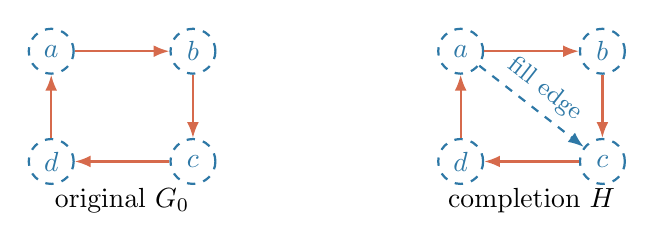
\begin{tikzpicture}[
  vertex/.style={circle,draw=navy,fill=white,minimum size=5.7mm,inner sep=0pt},
  arc/.style={-{Latex[length=2mm]},thick,orange},
  fill/.style={-{Latex[length=2mm]},thick,dashed,blue}]
  \node[vertex] (a) at (0,1.4) {$a$};
  \node[vertex] (b) at (1.8,1.4) {$b$};
  \node[vertex] (c) at (1.8,0) {$c$};
  \node[vertex] (d) at (0,0) {$d$};
  \draw[arc] (a)--(b); \draw[arc] (b)--(c);
  \draw[arc] (c)--(d); \draw[arc] (d)--(a);
  \node at (0.9,-0.5) {original $G_0$};

  \node[vertex] (a2) at (5.2,1.4) {$a$};
  \node[vertex] (b2) at (7,1.4) {$b$};
  \node[vertex] (c2) at (7,0) {$c$};
  \node[vertex] (d2) at (5.2,0) {$d$};
  \draw[arc] (a2)--(b2); \draw[arc] (b2)--(c2);
  \draw[arc] (c2)--(d2); \draw[arc] (d2)--(a2);
  \draw[fill] (a2)--node[above,sloped,font=\small] {fill edge} (c2);
  \node at (6.1,-0.5) {completion $H$};
\end{tikzpicture}
\caption{Triangle penalties cannot detect the directed four-cycle on the
left. The fill edge on the right is an ordering comparison only; either of its
directions produces a directed triangle.}
\label{fig:four-cycle}
\end{figure}

\subsection{Building the completion by elimination}

Begin with a temporary copy of $G_0$. Then repeat until it is empty:

\begin{enumerate}
  \item choose a remaining vertex $v$;
  \item find the neighbors of $v$ that are still present;
  \item add every missing edge needed to make those neighbors a clique; and
  \item record the added edges and remove $v$ from the temporary graph.
\end{enumerate}

Previously added fill edges count as ordinary connections in later steps. The
vertices are removed only from the temporary graph. The final graph $H$
contains every nonroot vertex, every original nonroot edge, and every recorded
fill edge. This construction guarantees that $H$ is chordal.

Different elimination orders produce different completions. We use a
deterministic minimum-fill heuristic: at each step, eliminate a vertex whose
remaining neighbors require the fewest new edges to become a clique. The
heuristic aims to keep $H$ small but is not guaranteed to find the smallest
completion.

\subsection{Ordering variables and Hamiltonian}

For each completion edge $\{u,v\}\in F$, with $u<v$, introduce one ordering
bit $x_{uv}$. There are no ordering variables for nonedges of $H$. The
selected-edge penalty remains Eq.~\eqref{eq:edge-order}, because it concerns
original selectable edges. Every original nonroot edge belongs to $H$, so its
required order variable exists. Fill edges have no $e$-variables and contribute
no cost.

For every triangle of $H$, use the polynomial in Eq.~\eqref{eq:triangle}:

\begin{equation}
F_{\mathrm{tri}}^{H}(x)=
\sum_{\substack{u<v<w\\
\{u,v\},\{u,w\},\{v,w\}\in F}}
\tau_{uvw}(x).
\label{eq:chordal-triangle}
\end{equation}

Using Fowler's unchanged parent terms gives

\begin{equation}
H_{\mathrm{CF}}(e,x)=\C(e)+P\left[
F_{\mathrm{tri}}^{H}+F_{\mathrm{edge}}+F_{\mathrm{term}}
+\sum_{v\in V\setminus T}F_v^{\mathrm F}\right].
\label{eq:chordal-fowler}
\end{equation}

Compared with Eq.~\eqref{eq:fowler}, only the ordering graph and the set of
triangles being checked have changed.

\subsection{A local nonterminal coefficient}

Chordal sparsification reduces variables and interactions but does not change
Fowler's coefficient $n$. We therefore study a second, independent
modification. Let $d_v^+$ be the number of allowed outgoing arcs from
nonterminal $v$, set $\alpha_v=d_v^++1$, and use

\begin{equation}
F_v^{\mathrm L}(e)=
\alpha_v\binom{q_v}{2}+(1-q_v)s_v.
\label{eq:local-parent}
\end{equation}

At $q_v=0$, the penalty is $s_v$; at $q_v=1$, it is zero. For $q_v\ge2$,

\begin{equation}
F_v^{\mathrm L}
=(q_v-1)\left(\frac{\alpha_vq_v}{2}-s_v\right)>0,
\label{eq:local-positive}
\end{equation}

because $s_v\le d_v^+<\alpha_v$. The local term therefore has exactly the same
zero states as Fowler's term. The choice $d_v^++1$ is tight for this form:
using $d_v^+$ could give zero at $q_v=2$ and $s_v=d_v^+$.

Replacing $F_v^{\mathrm F}$ in Eq.~\eqref{eq:chordal-fowler} by
$F_v^{\mathrm L}$ gives the chordal/local model $H_{\mathrm{CL}}$. This change
does not alter the QUBO variables or interaction locations; it changes only
their weights.

\section{Why the chordal formulation is exact}

The key question is whether checking only completion triangles can miss a long
directed cycle. Chordality rules this out.

\begin{lemma}
If an orientation of a chordal graph contains a directed cycle, then it
contains a directed triangle.
\end{lemma}

\begin{proof}
Choose a shortest directed cycle. If its length is at least four, chordality
provides an edge between two nonconsecutive cycle vertices. The cycle contains
a directed path between the two endpoints along each side. Whichever way the
chord is oriented, it closes one of these paths into a shorter directed cycle,
contradicting the choice of the original cycle. The shortest directed cycle
must therefore have length three.
\end{proof}

Consequently, $F_{\mathrm{tri}}^{H}=0$ makes the orientation of $H$ acyclic.
Since $F_{\mathrm{edge}}=0$ makes every selected nonroot arc follow this
orientation, selected nonroot arcs cannot cycle. A cycle containing $r$ is
also impossible because no selected arc enters $r$.

\begin{theorem}
An edge selection has a zero-penalty extension in the chordal/Fowler or
chordal/local model if and only if the selected arcs form a rooted
arborescence spanning every terminal, possibly with redundant nonterminal
leaves.
\end{theorem}

\begin{proof}
Suppose first that the total penalty is zero. Every nonroot terminal has one
parent by Eq.~\eqref{eq:terminal}. Every nonterminal with a child has one
parent, and no nonterminal has multiple parents, by
Eq.~\eqref{eq:fowler-parent} or Eq.~\eqref{eq:local-parent}. Selected arcs are
acyclic by the preceding argument.

Start at any selected nonroot vertex and repeatedly follow its incoming arc
backward. The chain cannot cycle. It cannot stop at a nonroot terminal because
every such terminal has a parent. It cannot stop at a nonterminal that has a
child because the nonterminal penalty gives that vertex a parent. The chain
must reach the root. All selected vertices lie in one rooted, acyclic component
that contains every terminal.

Conversely, take any Steiner tree and orient its edges away from $r$. Choose a
topological order of its vertices and orient every edge of $H$, including fill
edges, according to that order. All selected edges agree with the order, every
completion triangle is acyclic, and every parent penalty is zero. Hence every
valid Steiner tree has a zero-penalty extension.
\end{proof}

\subsection{A sufficient penalty weight}

All grouped penalties are nonnegative integers, with smallest positive value
at least one. If $U$ is the cost of any known feasible Steiner tree, then

\begin{equation}
P>U
\label{eq:penalty-bound}
\end{equation}

is sufficient for exact optimization. Every invalid assignment has energy at
least $P$, while a known valid assignment has energy at most $U$. Among valid
states the penalty is zero, so minimizing the Hamiltonian is exactly the same
as minimizing selected edge cost.

\section{Model size}

\subsection{Elimination width}

When a vertex is eliminated, count its neighbors that are still present in
the temporary graph. The \emph{width} $w$ of an elimination order is the
largest such count over all steps.

An eliminated vertex has at most $w$ later neighbors. It can therefore be
responsible for at most $w$ completion edges to later vertices and at most
$\binom{w}{2}$ completion triangles in which it is the earliest eliminated
vertex. If $Q=|F|$ and $\tau(H)$ is the number of triangles in $H$, then

\begin{equation}
Q=O(nw),
\qquad
\tau(H)=O(nw^2).
\label{eq:width-bounds}
\end{equation}

For bounded width, the ordering part grows linearly with $n$. In the worst
case $w=O(n)$, the completion can become complete and the chordal model reduces
to Fowler's asymptotic size. Sparse input alone does not guarantee small width.

\subsection{Comparison with complete ordering}

Let $a=2|E|-\deg_G(r)$ be the number of directed selection variables.

\begin{table}[ht]
\centering
\caption{The selected-edge and parent terms are common to both models.}
\label{tab:complexity}
\begin{tabular}{lcc}
\toprule
 & Complete order & Chordal order \\
\midrule
Ordering variables & $\binom{n-1}{2}$ & $Q$ \\
All binary variables & $a+\binom{n-1}{2}$ & $a+Q$ \\
Triangle constraints & $\binom{n-1}{3}$ & $\tau(H)$ \\
Triangle quadratic contributions & $3\binom{n-1}{3}$ & $3\tau(H)$ \\
\bottomrule
\end{tabular}
\end{table}

Figure~\ref{fig:size-ratio} shows measured BQM ratios on the 200-instance set
described in Section~\ref{sec:experiments}. Chordal/Fowler is compared with
Fowler so that only the ordering graph changes.

\begin{figure}[t]
\centering
\includegraphics[width=0.97\linewidth]{chordal_complexity_ratios.pdf}
\caption{Median chordal/Fowler BQM size divided by Fowler BQM size. Each point
summarizes ten instances. Lower values indicate a larger reduction.}
\label{fig:size-ratio}
\end{figure}

\section{Experimental evaluation}
\label{sec:experiments}

\subsection{Questions and compared models}

The experiments ask whether chordal ordering reduces model size, whether it
helps annealers reach valid trees, and whether observed changes come from
ordering sparsification or the local coefficient. We compare all four
combinations:

\begin{center}
\begin{tabular}{lll}
\toprule
Model & Ordering graph & Nonterminal coefficient \\
\midrule
Fowler & complete & $n$ \\
Full/local & complete & $d_v^++1$ \\
Chordal/Fowler & chordal completion & $n$ \\
Chordal/local & chordal completion & $d_v^++1$ \\
\bottomrule
\end{tabular}
\end{center}

Fowler versus chordal/Fowler isolates chordal sparsification. Full/local versus
chordal/local repeats this comparison with local parent weights. Comparisons
within one ordering type isolate the coefficient change.

\subsection{Method}

All reported runs use integer edge costs. We set
$P=\lceil1.05U\rceil$, where $U$ is the cost of a minimum spanning tree after
pruning nonterminal leaves. The optimum is never used to set $P$. Earlier
fractional-cost pilots are excluded because floating-point residue produced
degenerate automatic temperature ranges in Neal; no reported integer-cost run
had this problem.

Every model receives the same reads and sweeps. Each sample is decoded using
only its selected arcs and checked independently of auxiliary bits. A sample
is \emph{valid} when it is a rooted arborescence spanning every terminal, and
\emph{optimal} when its cost also equals the known optimum. Comparisons are
paired by instance, with bootstrap confidence intervals and Wilcoxon
signed-rank tests.

The main set contains 200 instances from five families: a spanning tree with
random extra edges, grids, geometric 4-nearest-neighbor graphs, and
Erd\H{o}s--R\'enyi graphs with probabilities $0.3$ and $0.6$. We use
$n\in\{8,12,16,20\}$, terminal fractions $25\%$ and $50\%$, and five seeds.
Neal and OpenJij simulated annealing receive 100 reads and 2,000 sweeps. A
larger set contains 150 instances with $n\in\{24,32,40\}$ and 5,000 sweeps.
We also test all 18 SteinLib B instances~\cite{koch2001}, with
$n\in\{50,75,100\}$, 100 reads, and 5,000 sweeps.

\subsection{Correctness checks}

On seven small graphs, including chordless four- and five-cycles, exhaustive
enumeration minimizes the penalty over all auxiliary assignments for every
selected-edge assignment. The minimum is zero exactly when the selected arcs
form a valid rooted tree, with no mismatches. Every observed penalty is a
nonnegative integer and the smallest positive penalty is one. All 23
formulation unit tests also pass.

\subsection{Generated instances}

Table~\ref{tab:general-rates} gives mean sample rates on the 200-instance set.
With Neal, changing only the ordering graph from complete to chordal raises
the valid rate by $6.8$ percentage points, with 95\% interval $[5.2,8.5]$.
Chordal/local improves the valid rate over Fowler by $7.3$ points, with
interval $[5.7,9.0]$, and the optimal rate by $1.2$ points, with interval
$[0.4,2.0]$. OpenJij shows the same main pattern.

\begin{table}[ht]
\centering
\caption{Mean sample rates on 200 generated instances, in percent.}
\label{tab:general-rates}
\begin{tabular}{lrrrr}
\toprule
& \multicolumn{2}{c}{Neal SA} & \multicolumn{2}{c}{OpenJij SA} \\
Model & Valid & Optimal & Valid & Optimal \\
\midrule
Fowler & 81.1 & 18.1 & 85.4 & 17.8 \\
Full/local & 82.1 & 18.6 & 85.2 & 19.9 \\
Chordal/Fowler & 87.9 & 19.1 & \textbf{90.9} & 20.4 \\
Chordal/local & \textbf{88.4} & \textbf{19.3} & 90.7 & \textbf{21.3} \\
\bottomrule
\end{tabular}
\end{table}

The gain depends strongly on graph structure. With Neal, chordal/local gains
$14.6$ valid-sample points on grids, $8.3$ on sparse graphs, $8.9$ on geometric
graphs, and $4.4$ on ER($0.3$). On dense ER($0.6$), where the chordal ordering
graph is $74\%$ of the complete graph, the gain is only $0.2$ point.

On the 150 larger instances, chordal/local gains $23.8$ valid-sample points
with Neal and $19.6$ with OpenJij. The gain grows as the completion becomes
smaller: for Neal, the Spearman correlation between size ratio and valid-rate
advantage is $\rho=-0.83$. Every model finds exact optima in fewer than $0.5\%$
of samples. Neal's best-tree gap improves by $7.4$ points, while the OpenJij
improvement is not statistically significant. In some geometric and dense
families, Fowler returns a better best tree despite chordal/local returning
many more valid trees. Validity and solution quality must be reported
separately.

\subsection{SteinLib B}

On all 18 SteinLib B instances, chordal/local produces more valid samples than
Fowler under both solvers. Fowler produces no valid tree in 8 of the 36
instance--solver runs, while chordal/local always produces at least one.
Chordal/local returns a better best tree on 15 of 18 instances with Neal and
10 of 18 with OpenJij. Across all 144 model--solver--instance runs, the exact
optimum is found once. Neither QUBO is a competitive exact Steiner solver at
this scale.

The chordal ordering graph has only $4$--$17\%$ as many edges as the complete
ordering graph, with measured widths from 4 to 22. Chordal/local uses 23--49
times fewer interactions and runs 10--25 times faster per annealing run.

\begin{table}[ht]
\centering
\caption{Representative SteinLib B sizes and Neal run times. Each entry is
Fowler / chordal-local.}
\label{tab:steinlib-size}
\begin{tabular}{rrrr}
\toprule
$n$ & Variables & Interactions & Seconds per run \\
\midrule
50  & 1,373 / 396 & 56,377 / 2,413 & 32 / 3 \\
75  & 2,997 / 672 & 196,014 / 5,364 & 97 / 6 \\
100 & 5,244 / 965 & 472,577 / 9,578 & 318 / 13 \\
\bottomrule
\end{tabular}
\end{table}

\subsection{Coefficient normalization}

We also run untuned OpenJij simulated quantum annealing after normalizing each
Ising model to maximum absolute bias one. All models perform poorly: valid
rates are $1.5$--$4.3\%$ and are near zero for $n\ge16$. Chordal/Fowler does
not improve on Fowler in this setting, while both local-coefficient models do.
Normalization by Fowler's $nP$ scale compresses the other energy differences;
the degree-local coefficient reduces this effect. This supports the
coefficient change as an independent scaling improvement, but it is not
evidence about quantum hardware.

\section{Discussion and limitations}

The theoretical contribution is exact: chordal ordering changes the auxiliary
acyclicity certificate without changing the valid selected-edge set. Its size
advantage is instance-dependent. When elimination width is small, the
completion can be much smaller than a complete graph. When width is large, the
method approaches Fowler's model. Root choice and elimination order can
therefore influence the final QUBO.

The experimental advantage is clearest in model size, sampling time, and the
probability of obtaining a valid tree. Best-tree quality is less consistent.
Removing interactions changes the energy landscape and does not uniformly
improve optimization.

The experiments use one penalty factor and one sweep budget per instance size.
No sensitivity study is included. Equal sweeps are not equal time because
chordal models are often faster; an equal-time comparison remains important.
We perform no quantum-hardware runs, minor-embedding study, or comparison with
modern classical Steiner solvers. The results concern QUBO representation and
heuristic sampling, not quantum advantage or competitive exact optimization.

\section{Conclusion}

The complete-order Steiner QUBO prevents cycles by comparing every pair of
nonroot vertices. The chordal formulation keeps the same selected-edge and
parent logic but stores only the comparisons needed on a chordal completion.
Fill edges belong only to the auxiliary ordering graph: they carry no cost and
cannot be selected into the tree. Since every cyclic orientation of a chordal
graph contains a directed triangle, local triangle penalties enforce global
acyclicity.

For elimination width $w$, the ordering part has $O(nw)$ variables and
$O(nw^2)$ triangle interactions, with the complete graph as its worst case.
The degree-local coefficient separately reduces Fowler's global multiplier
without changing feasible states. Experiments show large size and valid-sample
improvements when the completion is small, but no universal improvement in
best-tree cost.

\paragraph{Reproducibility.}
The implementation, tests, benchmark scripts, and result files are available
at \url{https://github.com/daghanerdonmez/finale}. The principal formulation is
in \path{research/steiner_to_bqm_chordal.py}; the generated-instance and
SteinLib experiments are in \path{benchmark_general.py} and
\path{benchmark_steinlib.py}.

\begin{thebibliography}{99}

\bibitem{hwang1992}
F. K. Hwang, D. S. Richards, and P. Winter,
\emph{The Steiner Tree Problem}. North-Holland, 1992.

\bibitem{karp1972}
R. M. Karp,
``Reducibility among combinatorial problems,'' in
\emph{Complexity of Computer Computations}, R. E. Miller and
J. W. Thatcher, Eds. Plenum Press, pp.~85--103, 1972.
\href{https://doi.org/10.1007/978-1-4684-2001-2_9}{doi:10.1007/978-1-4684-2001-2\_9}.

\bibitem{glover2019}
F. Glover, G. Kochenberger, and Y. Du,
``Quantum bridge analytics I: A tutorial on formulating and using QUBO
models,'' \emph{4OR}, vol.~17, no.~4, pp.~335--371, 2019.
\href{https://doi.org/10.1007/s10288-019-00424-y}{doi:10.1007/s10288-019-00424-y}.

\bibitem{lucas2014}
A. Lucas,
``Ising formulations of many NP problems,''
\emph{Frontiers in Physics}, vol.~2, art.~5, 2014.
\href{https://doi.org/10.3389/fphy.2014.00005}{doi:10.3389/fphy.2014.00005}.

\bibitem{fowler2017}
A. Fowler,
``Improved QUBO formulations for D-Wave quantum computing,''
technical report, University of Auckland, 2017.
\href{https://doi.org/10.13140/RG.2.2.31829.73445}{doi:10.13140/RG.2.2.31829.73445}.

\bibitem{rose1976}
D. J. Rose, R. E. Tarjan, and G. S. Lueker,
``Algorithmic aspects of vertex elimination on graphs,''
\emph{SIAM Journal on Computing}, vol.~5, no.~2, pp.~266--283, 1976.
\href{https://doi.org/10.1137/0205021}{doi:10.1137/0205021}.

\bibitem{rankooh2022}
M. F. Rankooh and J. Rintanen,
``Propositional encodings of acyclicity and reachability by using vertex
elimination,'' in \emph{Proceedings of AAAI}, vol.~36, no.~5,
pp.~5861--5868, 2022.
\href{https://doi.org/10.1609/aaai.v36i5.20530}{doi:10.1609/aaai.v36i5.20530}.

\bibitem{koch2001}
T. Koch, A. Martin, and S. Vo\ss,
``SteinLib: An updated library on Steiner tree problems in graphs,''
in \emph{Steiner Trees in Industries}, D.-Z. Du and X. Cheng, Eds.
Kluwer, pp.~285--325, 2001.
\href{https://doi.org/10.1007/978-1-4613-0255-1_9}{doi:10.1007/978-1-4613-0255-1\_9}.

\end{thebibliography}

\end{document}
